\documentclass[11pt,titlepage]{article}
\usepackage[margin=1.0in]{geometry}
\usepackage[T1]{fontenc}
\usepackage[utf8]{inputenc}
\usepackage{amsmath,amssymb,amsthm}
\usepackage{booktabs}
\usepackage{array}
\usepackage{longtable}
\usepackage{graphicx}
\graphicspath{{figures/}}
\usepackage[hypertexnames=false]{hyperref}
\usepackage{xcolor}
\usepackage{url}
\usepackage{float}
\usepackage{algorithm}
\usepackage{algpseudocode}
\hypersetup{colorlinks=true,linkcolor=darkgray,citecolor=blue,urlcolor=blue}
\emergencystretch=2em

\newcommand{\systemu}{ELARA-U}
\newcommand{\system}{ELARA}
\newcommand{\method}{RGA}
\newcommand{\methodplus}{RGA+}
\newcommand{\gateu}{Gate U}
\newcommand{\relg}{\textsc{RelGate}}
\newcolumntype{L}[1]{>{\raggedright\arraybackslash}p{#1}}

% Theorem-like environments
\ifcsname c@theorem\endcsname\else\newtheorem{theorem}{Theorem}\fi
\ifcsname c@corollary\endcsname\else\newtheorem{corollary}{Corollary}\fi
\ifcsname c@proposition\endcsname\else\newtheorem{proposition}{Proposition}\fi
\ifcsname c@lemma\endcsname\else\newtheorem{lemma}{Lemma}\fi
\ifcsname c@certificate\endcsname\else\newtheorem{certificate}{Certificate}\fi
\ifcsname c@diagnostic\endcsname\else\newtheorem{diagnostic}{Diagnostic}\fi
\ifcsname c@slack\endcsname\else\newtheorem{slack}{Proposition}\fi

\begin{document}

\begin{titlepage}
\centering
\vspace*{1.7cm}
{\huge\bfseries ELARA-U: A Cross-Domain Anomaly Meta-Routing Benchmark\\ ---Stacking Beats Selection; Reliability Routing Does Not\par}
\vspace{1.4cm}
{\large\bfseries Pratik Niroula}\par
\vspace{0.4cm}
{\large Independent Researcher}\par
\vspace{1.8cm}
{\Large\itshape Expanded Thesis Chapter and Research Monograph\par}
\vspace{1.5cm}
{\large \today\par}
\vspace{1.6cm}
\begin{minipage}{0.86\linewidth}
\small
\textbf{Thesis statement.} The central problem in universal anomaly detection is
not only inventing a stronger detector, but preventing the wrong detector from
being trusted under domain shift. \systemu{} studies this as a meta-routing
problem: given a heterogeneous detector zoo and a validation slice, decide when
to select, fuse, stack, or fall back without using test labels. On the clean i.i.d.\ archive of
$123$ tasks from $5$ families, \systemu{} Stack (per-task rank-normalized
stacking) reaches mean rank $2.53$ versus $3.38$ for validation auto-selection
($+0.036$ AUROC, paired-bootstrap CI $[+0.023,+0.050]$, excluding zero; $86/123$
wins) and even exceeds the best-single-detector oracle ($0.784$ vs $0.756$). However,
controlled ablations across four regimes (Holm-corrected) and a \emph{sealed natural
temporal-shift} benchmark (D22) resolve RQ3 negatively: reliability/drift features add
no significant value in any regime, and a reliability gate on the stack is significantly
\emph{worse} ($-0.037$ AUROC, $p_{\mathrm{Holm}}{<}10^{-8}$); under natural shift the
drift router is directionally worse ($-0.050$ AUROC, raw CI excl.\ $0$, but $n{=}7$ does
not survive Holm). The honest contribution is a cross-domain benchmark with a strong
stacking baseline and a Holm-robust negative result for reliability-aware
routing---not a sealed universal SOTA claim.
\end{minipage}
\end{titlepage}

\tableofcontents
\listoftables
\listoffigures
\newpage

\section{Executive Summary}

Anomaly detection is fragmented across tabular, cyber, fraud, image-OOD, text,
industrial vision, time-series, and multimodal settings. Each family has strong
specialists, but none is uniformly best. In deployment, the damaging failure is
often not the absence of a useful expert; it is selecting a detector whose
validation performance no longer predicts deployment performance. This is the
negative-transfer problem.

\systemu{} reframes the project around a universal anomaly \emph{meta-router}.
Instead of claiming that one detector is universal, \systemu{} asks whether a
router can reduce average rank, regret to the per-task oracle, and harmful
transfer events across many task families. The project therefore moves from the
old clean-transfer-only framing to a broader \gateu{} contract: success is judged
by cross-family rank, regret, calibration, negative-transfer reduction, and
audited no-test-label routing.

\subsection{Current Evidence Level}

The current thesis evidence should be read in three tiers.

\begin{table}[H]
\centering
\caption{Evidence status of the current ELARA-U thesis.}
\label{tab:evidence-status}
\small
\begin{tabular}{L{0.25\linewidth}L{0.43\linewidth}L{0.22\linewidth}}
\toprule
\textbf{Evidence tier} & \textbf{What it shows} & \textbf{Claim status} \\
\midrule
Clean 123-task benchmark & Rank-normalized stacking beats validation auto-select ($+0.036$ AUROC, CI$>$0) and the best fixed detector ($+0.075$) across 5 families. & Established (verified) \\
Reliability ablation & Reliability/drift features add no significant gain over validation quality; a reliability gate hurts. & Established (negative) \\
Mechanism (simulation) & Reliability gating helps iff a channel fails independently. & Established (simulation) \\
Natural multimodal / sealed holdout & The regime where reliability should structurally help; pre-registered. & Pending \\
\bottomrule
\end{tabular}
\end{table}

The immediate research value is that the work now has a defensible thesis:
\emph{meta-routing is most useful when validation metrics become stale under
deployment shift}. This is stronger and cleaner than claiming one fixed detector
or one clean-transfer gate should win everywhere.

\section{Research Questions and Contributions}

\subsection{Research Questions}

\begin{table}[H]
\centering
\caption{Core research questions for the ELARA-U thesis.}
\label{tab:rq}
\small
\begin{tabular}{L{0.08\linewidth}L{0.56\linewidth}L{0.24\linewidth}}
\toprule
\textbf{ID} & \textbf{Question} & \textbf{Current status} \\
\midrule
RQ1 & Can a cross-domain router outperform the best fixed detector family over many anomaly tasks? & Yes (clean 123-task benchmark, CI$>$0) \\
RQ2 & Can the router (stack) outperform validation-AUROC auto-selection? & Yes ($+0.036$ AUROC, CI$>$0) \\
RQ3 & Does reliability/drift modeling, rather than plain stacking, carry the improvement? & \textbf{Resolved: NO} (3 regimes, 2 designs; Table~\ref{tab:ablation}) \\
RQ4 & Can the same contract hold on natural, sealed, and external benchmarks (incl.\ multimodal)? & Pending; pre-registered (Sec.~\ref{sec:multimodal}) \\
RQ5 & Can the router produce calibrated probabilities and safe abstentions suitable for operations? & Partially supported; calibration pending \\
\bottomrule
\end{tabular}
\end{table}

\subsection{Contributions}

\begin{longtable}{L{0.22\linewidth}L{0.47\linewidth}L{0.22\linewidth}}
\caption{Contribution matrix.}\label{tab:contrib}\\
\toprule
\textbf{Contribution} & \textbf{Description} & \textbf{Evidence} \\
\midrule
\endfirsthead
\toprule
\textbf{Contribution} & \textbf{Description} & \textbf{Evidence} \\
\midrule
\endhead
Universal meta-routing formulation & Defines anomaly detection as a task-level routing problem over a detector zoo, not as a single-detector competition. & Formal setup and \gateu{} \\
Score archive & Persists validation/test detector scores, labels, and provenance so routing policies can be evaluated without re-running detectors. & $123$ current tasks \\
Rank-normalized stacker & Learns per-task combinations from validation labels and applies monotone-invariant rank features to test scores. & Mean rank $2.53$ (clean benchmark) \\
Evidence contract & Separates average rank, regret, negative transfer, calibration, and no-test-label audit. & Tables and algorithms \\
Theory stack & Proves why universal dominance is impossible, why auto-select is near-oracle under stable transfer, and why shifted regimes can reward reliability routing. & Theorems in Sec.~\ref{sec:theory} \\
Honest boundary & Distinguishes development stress evidence from sealed universal SOTA evidence. & Validity audit \\
\bottomrule
\end{longtable}

\section{Problem Definition}

Let $\mathcal{T}$ be a collection of anomaly-detection tasks. Each task
$\tau\in\mathcal{T}$ has a training split, a validation split, and a deployment or
test split. A detector zoo
\[
\mathcal{D}=\{d_1,\ldots,d_M\}
\]
produces detector scores $s_{\tau,m}(x)$ for every sample $x$. The objective is
not to find a detector that wins every task. The objective is to learn or define a
router $R$ that maps task evidence into a selected, fused, or stacked score
\[
g_\tau(x)=R\left(\{s_{\tau,m}\}_{m=1}^{M}, \Phi_\tau\right)(x),
\]
where $\Phi_\tau$ contains validation-only and unlabeled deployment-shift
features. The router is evaluated using test labels only after routing decisions
are frozen.

\subsection{Metrics}

\begin{table}[H]
\centering
\caption{Primary metrics used by the thesis.}
\label{tab:metrics}
\small
\begin{tabular}{L{0.25\linewidth}L{0.47\linewidth}L{0.20\linewidth}}
\toprule
\textbf{Metric} & \textbf{Definition} & \textbf{Preferred direction} \\
\midrule
Mean rank & Average rank of each method by task AUROC. & Lower \\
Regret & Per-task oracle AUROC minus method AUROC. & Lower \\
Negative-transfer rate & Fraction of tasks where the method underperforms a safe reference such as rank-mean. & Lower \\
Bootstrap CI & Paired task-level confidence interval for rank delta. & Exclude zero \\
ECE proxy & Calibration error treating normalized scores as probabilities. & Lower \\
Worst rank/regret & Worst observed task-level failure. & Lower \\
\bottomrule
\end{tabular}
\end{table}

\section{From the Old ELARA System to ELARA-U}

The prior \system{}/\method{} work remains useful, but it should be treated as
source-system evidence rather than the main flagship claim. Its value is threefold:
it provides a detector-and-fusion foundation, it supplies negative evidence about
near-ceiling clean transfer, and it motivates a broader meta-routing benchmark.

\begin{table}[H]
\centering
\caption{How old artifacts should be reused in the new thesis.}
\label{tab:reuse}
\small
\begin{tabular}{L{0.24\linewidth}L{0.42\linewidth}L{0.24\linewidth}}
\toprule
\textbf{Old artifact} & \textbf{Reuse in ELARA-U} & \textbf{Do not use as} \\
\midrule
RGA/RGA+ source system & Detector/fusion foundation and stress mechanism. & Universal proof \\
Clean-transfer failures & Motivation for the new routing objective. & A hidden pass \\
T1--T9 theory stack & Boundary theorems explaining when clean transfer is hard. & A reason to overclaim \\
Real-IAD / Real-IAD D3 & Natural-degradation evidence track and future family input. & Fresh sealed evidence if already opened \\
MVTec 3D-AD / 3D-ADAM / MulSen & Multimodal source families and development evidence. & Final universal holdout without preregistration \\
\bottomrule
\end{tabular}
\end{table}

This distinction is important. A failed clean-transfer gate does not make the
project worthless; it says that the old claim was too narrow. The stronger
scientific move is to make the failure part of the motivation: when clean
validation-to-test transfer is stable, validation auto-selection is already a
strong baseline. A universal paper should therefore focus on the regimes where
selection becomes stale.

\section{Methodology: The Reliability-Aware Meta-Router}

\systemu{} operates in two conceptually distinct modes.

\begin{table}[H]
\centering
\caption{ELARA-U operating modes.}
\label{tab:modes}
\small
\begin{tabular}{L{0.20\linewidth}L{0.42\linewidth}L{0.26\linewidth}}
\toprule
\textbf{Mode} & \textbf{Behavior} & \textbf{Best use} \\
\midrule
Clean baseline mode & Select the detector with highest validation AUROC. & Stable validation-to-test transfer \\
Shift-aware stack mode & Fit a regularized rank-normalized stacker on validation data and apply it to test ranks. & Stale validation under score shift or degradation \\
Fallback mode & Use rank-mean or abstain when channels are degenerate. & Unsafe or untrusted routing \\
\bottomrule
\end{tabular}
\end{table}

\subsection{Detector Zoo and Router Features}

\begin{table}[H]
\centering
\caption{Detector zoo. Current archive uses the tabular/cyber/fraud/image/text subsets; the remaining families are thesis expansion targets.}
\label{tab:zoo}
\small
\begin{tabular}{L{0.22\linewidth}L{0.62\linewidth}}
\toprule
\textbf{Domain} & \textbf{Experts} \\
\midrule
Tabular & ECOD, COPOD, Isolation Forest, LOF, KNN, OCSVM \\
Cyber/fraud & One-class and density detectors over transaction or network features \\
Image-OOD & Feature-space anomaly detectors over CNN representations \\
Text & Feature-space anomaly detectors over sentence/document embeddings \\
Time series & Matrix profile, forecasting residual, reconstruction, and sequence models \\
Industrial vision & PatchCore, reverse-distillation, EfficientAD-style experts \\
Multimodal/3D & RGB, depth, point-cloud, SAR/CW-style multimodal fusions \\
\bottomrule
\end{tabular}
\end{table}

\begin{table}[H]
\centering
\caption{Router feature families.}
\label{tab:feat}
\small
\begin{tabular}{L{0.22\linewidth}L{0.50\linewidth}L{0.18\linewidth}}
\toprule
\textbf{Group} & \textbf{Examples} & \textbf{Labels} \\
\midrule
Validation reliability & validation AUROC, spread, confidence, inversion flags & validation only \\
Score geometry & entropy, sharpness, tail mass, saturation, rank dispersion & no labels \\
Disagreement & inter-expert rank and score disagreement & no labels \\
Shift & validation-to-test KS drift, score distribution drift & no test labels \\
Dataset meta-features & sample count, dimension, anomaly rate on validation & validation only \\
Calibration & ECE proxy, future Brier/NLL after fitted calibration & validation only \\
\bottomrule
\end{tabular}
\end{table}

% ELARA: main algorithms + theorem/certificate boxes.
% Include file for the ELARA flagship manuscript. Host preamble must load:
%   \usepackage{amsmath,amssymb,amsthm,algorithm,algpseudocode}
% and define theorem-like environments (provided here if not already defined).
%
% Algorithms mirror the real harness src/scripts/elara_u/gate_u_seed_eval.py and
% the Gate U protocol research_lock/GATE_U_CROSS_DOMAIN_PROTOCOL_v1.yaml.

% ---- theorem-like environments (guarded so double-definition is harmless) ----
\ifcsname c@certificate\endcsname\else\newtheorem{certificate}{Certificate}\fi
\ifcsname c@diagnostic\endcsname\else\newtheorem{diagnostic}{Diagnostic}\fi
\ifcsname c@slack\endcsname\else\newtheorem{slack}{Proposition}\fi

% =====================================================================
% Algorithm 1: Universal Score Archive Construction
% =====================================================================
\begin{algorithm}[t]
\caption{Universal Score Archive Construction}
\label{alg:archive}
\begin{algorithmic}[1]
\Require datasets $\mathcal{D}=\{X_d\}$, detector zoo $\mathcal{E}=\{e_1,\dots,e_M\}$
\Ensure score archive $\mathcal{A}$, validation summaries $V$
\For{each dataset $d \in \mathcal{D}$}
  \State split $X_d$ into $\mathrm{train}/\mathrm{val}/\mathrm{test}$; fit scaler on train
  \For{each expert $e_m \in \mathcal{E}$}
    \State fit $e_m$ on (unlabelled) train; $s^{\mathrm{val}}_{d,m}\!\gets\! e_m(\mathrm{val})$, $s^{\mathrm{test}}_{d,m}\!\gets\! e_m(\mathrm{test})$
    \State normalise by monotone $z$-sigmoid on the train-OK score distribution
    \State $v_{d,m} \gets \mathrm{AUROC}(y_{\mathrm{val}}, s^{\mathrm{val}}_{d,m})$ \Comment{validation labels only}
    \State store $(s^{\mathrm{val}}_{d,m}, s^{\mathrm{test}}_{d,m}, v_{d,m})$ and provenance (config hash, artifact hash) in $\mathcal{A}$
  \EndFor
\EndFor
\State \Return $\mathcal{A}$, $V=\{v_{d,m}\}$
\end{algorithmic}
\end{algorithm}

% =====================================================================
% Algorithm 2: Validation-Only Reliability Router Training
% =====================================================================
\begin{algorithm}[t]
\caption{Validation-Only Reliability Router Training}
\label{alg:router-train}
\begin{algorithmic}[1]
\Require archive $\mathcal{A}$, validation summaries $V$, dataset meta-features $\Phi$
\Ensure frozen router $R$
\For{each $(d,m)$}
  \State $r_{d,m} \gets [\,$score tailness, entropy, inter-expert disagreement, calibration error,
  \Statex \hspace{2.2em} missing-modality flags, domain-shift estimate, $v_{d,m}$, $\Phi_d\,]$ \Comment{no test labels}
\EndFor
\State target $t_d \gets \arg\max_m v_{d,m}$ (or the per-dataset rank vector)
\State fit $R:\; r \mapsto$ (expert choice / fusion weights) on $\{(r_{d,\cdot}, t_d)\}$ using validation only
\State \textbf{audit:} assert no test split or test label entered $R$'s fit
\State \Return frozen $R$
\end{algorithmic}
\end{algorithm}

% =====================================================================
% Algorithm 3: Routed Inference With Abstention
% =====================================================================
\begin{algorithm}[t]
\caption{Routed Inference With Abstention}
\label{alg:route-infer}
\begin{algorithmic}[1]
\Require frozen router $R$, calibrator $g$, abstention threshold $\tau_a$, new task scores $\{s_m\}$ with validation slice
\Ensure calibrated routed score or abstention, with reason code
\State $r \gets$ reliability features on the task's validation slice (Alg.~\ref{alg:router-train})
\State $(\,w, \hat{\rho}\,) \gets R(r)$ \Comment{fusion weights $w$ and predicted reliability $\hat{\rho}$}
\If{$\hat{\rho} < \tau_a$ \textbf{or} all experts flagged degenerate}
  \State \Return \textsc{Abstain} with reason code (low predicted reliability)
\EndIf
\State $\tilde{s} \gets \sum_m w_m\, s_m$ over non-degenerate experts (degenerate-channel guard)
\State \Return $g(\tilde{s})$ (calibrated) with reason code (selected experts, weights)
\end{algorithmic}
\end{algorithm}

% =====================================================================
% Algorithm 4 (appendix): Universal Evidence Evaluation
% =====================================================================
\begin{algorithm}[t]
\caption{Universal Evidence Evaluation (Gate U)}
\label{alg:gate-u}
\begin{algorithmic}[1]
\Require per-task test AUROCs for router and baselines over tasks $\mathcal{T}$
\Ensure Gate U evidence report
\For{each task $\tau \in \mathcal{T}$}
  \State rank methods by test AUROC; $\mathrm{oracle}_\tau \gets \max$ AUROC
  \State $\mathrm{regret}_\tau(\cdot) \gets \mathrm{oracle}_\tau - \mathrm{AUROC}_\tau(\cdot)$; flag negative transfer vs best fixed
\EndFor
\State aggregate mean rank, win rate, mean/worst regret, negative-transfer rate
\State paired bootstrap over $\mathcal{T}$ for (router $-$ best-fixed) rank gain $\Rightarrow$ 95\% CI
\State Holm-correct across the endpoint family; \Return report
\end{algorithmic}
\end{algorithm}

% Theorem / certificate boxes have been moved to the appendix (ELARA_U_THEORY_APPENDIX.tex)



\section{Theory Stack}
\label{sec:theory-intro}

The theory stack is not a proof that \systemu{} is universal SOTA. It is a proof
of when the claim is possible and when it is structurally impossible. The key
message is:
\[
\text{ELARA-U helps when stale-validation regret } \Delta \text{ exceeds router prediction error } 2\eta.
\]
If validation and deployment detector rankings remain stable, auto-selection is
already near-oracle. If deployment shift changes detector ranking and the router
can predict that change from validation-only and unlabeled shift evidence, routing
can reduce regret.

\section{Theory Stack for ELARA-U: Shift-Aware Reliability Routing}
\label{sec:theory}

\subsection{Notation and Setup}

Let $\mathcal{D}=\{1,\ldots,M\}$ be a finite detector zoo. For a task $\tau$, detector $m\in\mathcal{D}$ produces an anomaly score $s_m(x)\in \mathbb{R}$. Let $V_\tau$ denote the validation distribution and $T_\tau$ denote the deployment/test distribution. Let
\[
A_V(m)=\mathrm{AUROC}_{V_\tau}(s_m), \qquad
A_T(m)=\mathrm{AUROC}_{T_\tau}(s_m).
\]
The validation auto-selector is
\[
m_{\mathrm{val}} = \arg\max_{m\in\mathcal{D}} A_V(m),
\]
and the test oracle is
\[
m^\star = \arg\max_{m\in\mathcal{D}} A_T(m).
\]
The test regret of a method $h$ is
\[
\mathrm{Reg}_T(h)=A_T(m^\star)-A_T(h).
\]
When $h$ outputs a fused or stacked score $g_h(x)$ instead of a single detector, define
\[
A_T(h)=\mathrm{AUROC}_{T_\tau}(g_h).
\]
ELARA-U observes validation-only reliability features and unlabeled deployment-shift features, including score dispersion, entropy, inter-detector disagreement, calibration error, detector degeneracy flags, and train-validation/test-score drift statistics. It never observes test labels during routing.

\subsection{Main Evidentiary Theorems}

\begin{theorem}[No Universal Dominance Without Assumptions]
\label{thm:universal_dominance}
For any deterministic detector, fusion rule, or meta-router $h$ that selects or combines scores from a finite detector zoo $\mathcal{D}$, there exists a pair of anomaly-detection tasks $(\tau_1,\tau_2)$ such that $h$ cannot be strictly optimal on both tasks. Therefore, no universal anomaly detector or router can dominate all alternatives across all possible domains without assumptions on task structure, reliability, or shift.
\end{theorem}
\begin{proof}
Fix any method $h$. Since $h$ is deterministic, for a given task representation it outputs either one detector or a fixed scoring function $g_h$ built from detector scores.

Construct a task $\tau_1$ where $g_h$ ranks all anomalous examples above all normal examples. Then
\[
A_{\tau_1}(h)=1.
\]
Now construct a second task $\tau_2$ on the same score space by reversing the anomaly labels: all examples ranked high by $g_h$ are normal and all examples ranked low by $g_h$ are anomalous. Under this label reversal,
\[
A_{\tau_2}(h)=0.
\]
However, there exists another detector $m'$ that ranks the $\tau_2$ anomalies above normals, achieving
\[
A_{\tau_2}(m')=1.
\]
\end{proof}
Thus $h$ is optimal on $\tau_1$ but maximally suboptimal on $\tau_2$. Since this construction can be made for any fixed $h$, no detector, fusion rule, or router can be universally dominant without additional assumptions.

\medskip
\noindent\textbf{Interpretation.}
This theorem justifies the ELARA-U claim structure: the paper does not claim ``best on every dataset.'' The defensible claim is reduction of regret and negative transfer under specified reliability and shift conditions.

\begin{theorem}[Validation Auto-Selection Is Near-Oracle Under Stable Transfer]
\label{thm:stable_transfer}
Assume validation and deployment detector performances are uniformly close:
\[
\sup_{m\in\mathcal{D}} |A_T(m)-A_V(m)| \leq \varepsilon.
\]
Then validation-AUROC auto-selection has deployment regret bounded by
\[
\mathrm{Reg}_T(m_{\mathrm{val}}) \leq 2\varepsilon.
\]
\end{theorem}
\begin{proof}
Let $m^\star=\arg\max_{m}A_T(m)$ be the test oracle. By definition of $m_{\mathrm{val}}$,
\[
A_V(m_{\mathrm{val}})\geq A_V(m^\star).
\]
Using the uniform stability assumption,
\[
A_T(m_{\mathrm{val}})\geq A_V(m_{\mathrm{val}})-\varepsilon,
\]
and
\[
A_V(m^\star)\geq A_T(m^\star)-\varepsilon.
\]
Combining these inequalities gives
\[
A_T(m_{\mathrm{val}})
\geq A_V(m_{\mathrm{val}})-\varepsilon
\geq A_V(m^\star)-\varepsilon
\geq A_T(m^\star)-2\varepsilon.
\]
Therefore,
\[
\mathrm{Reg}_T(m_{\mathrm{val}}) = A_T(m^\star)-A_T(m_{\mathrm{val}}) \leq 2\varepsilon.
\]
\end{proof}

\medskip
\noindent\textbf{Interpretation.}
This theorem explains why validation-AUROC auto-selection is hard to beat on clean i.i.d. validation-to-test transfer. If validation and deployment rankings match, auto-select is already near-oracle.

\begin{theorem}[Stale Validation Causes Auto-Selection Failure Under Shift]
\label{thm:stale_validation}
There exist shifted deployment settings where validation auto-selection incurs arbitrarily large regret up to the AUROC range. In particular, for any $\gamma>0$ and any $\Delta>0$ such that the AUROC values remain in $[0,1]$, there exists a two-detector task with
\[
A_V(1)=a+\gamma,\qquad A_V(2)=a,
\]
but
\[
A_T(1)=a-\Delta,\qquad A_T(2)=a.
\]
Then validation auto-selection chooses detector 1, while the deployment oracle chooses detector 2, and the regret is
\[
\mathrm{Reg}_T(m_{\mathrm{val}})=\Delta.
\]
\end{theorem}
\begin{proof}
Because $A_V(1)=a+\gamma>A_V(2)=a$, validation auto-selection chooses $m_{\mathrm{val}}=1$. At deployment time, however, $A_T(2)=a>A_T(1)=a-\Delta$, so the test oracle is $m^\star=2$. Therefore,
\[
\mathrm{Reg}_T(m_{\mathrm{val}}) = A_T(m^\star)-A_T(m_{\mathrm{val}}) = A_T(2)-A_T(1) = a-(a-\Delta) = \Delta.
\]
Since $\Delta$ can be made large subject only to the AUROC range $[0,1]$, stale validation can cause large auto-selection regret.
\end{proof}

\medskip
\noindent\textbf{Interpretation.}
This theorem formalizes the main ELARA-U motivation: validation auto-selection can be near-oracle when validation and test match, but it can fail badly when deployment shift changes the detector ranking.

\begin{theorem}[Reliability-Separation Improvement Over Stale Auto-Selection]
\label{thm:reliability_separation}
Suppose ELARA-U constructs a reliability predictor $\widehat{A}_T(m)$ for deployment performance using validation-only reliability features and unlabeled deployment-shift features. Assume the predictor is uniformly accurate:
\[
\sup_{m\in\mathcal{D}} |\widehat{A}_T(m)-A_T(m)| \leq \eta.
\]
Let $m_R=\arg\max_{m\in\mathcal{D}}\widehat{A}_T(m)$ be the reliability-routed choice. Then
\[
\mathrm{Reg}_T(m_R)\leq 2\eta.
\]
Moreover, if stale validation auto-selection has regret
\[
\mathrm{Reg}_T(m_{\mathrm{val}}) > 2\eta,
\]
then the reliability router strictly improves over validation auto-selection by at least
\[
\mathrm{Reg}_T(m_{\mathrm{val}})-2\eta.
\]
\end{theorem}
\begin{proof}
Let $m^\star=\arg\max_m A_T(m)$ be the test oracle. Since $m_R$ maximizes $\widehat{A}_T(m)$,
\[
\widehat{A}_T(m_R)\geq \widehat{A}_T(m^\star).
\]
Using the uniform prediction-error assumption,
\[
A_T(m_R)\geq \widehat{A}_T(m_R)-\eta,
\]
and
\[
\widehat{A}_T(m^\star)\geq A_T(m^\star)-\eta.
\]
Combining,
\[
A_T(m_R)
\geq \widehat{A}_T(m_R)-\eta
\geq \widehat{A}_T(m^\star)-\eta
\geq A_T(m^\star)-2\eta.
\]
Therefore,
\[
\mathrm{Reg}_T(m_R) = A_T(m^\star)-A_T(m_R) \leq 2\eta.
\]
If $\mathrm{Reg}_T(m_{\mathrm{val}})>2\eta$, then
\[
\mathrm{Reg}_T(m_{\mathrm{val}})-\mathrm{Reg}_T(m_R) \geq \mathrm{Reg}_T(m_{\mathrm{val}})-2\eta > 0.
\]
Thus the reliability router strictly improves over stale validation auto-selection.
\end{proof}

\medskip
\noindent\textbf{Interpretation.}
This is the main positive theorem. ELARA-U can beat auto-select only when its reliability and drift features predict shifted deployment performance better than stale validation AUROC does.

\begin{theorem}[Safe Switching and Fallback Bound]
\label{thm:safe_switching}
Let $\Delta_{\mathrm{fired}} = A_T(h_{\mathrm{route}})-A_T(h_{\mathrm{default}})$ be the performance gain of routing over a default method on the subset of tasks or inputs where the router fires. Suppose ELARA-U switches away from the default only when a valid one-sided $(1-\alpha)$-confidence lower bound satisfies
\[
\mathrm{LCB}_{1-\alpha}(\Delta_{\mathrm{fired}})>0.
\]
Then, with probability at least $1-\alpha$, every admitted switch has non-negative true improvement:
\[
\Delta_{\mathrm{fired}}>0.
\]
Equivalently, the probability that ELARA-U admits a harmful switch is at most $\alpha$.
\end{theorem}
\begin{proof}
By validity of the one-sided confidence bound,
\[
\Pr\left(\mathrm{LCB}_{1-\alpha}(\Delta_{\mathrm{fired}})\leq \Delta_{\mathrm{fired}}\right)\geq 1-\alpha.
\]
ELARA-U admits a switch only if $\mathrm{LCB}_{1-\alpha}(\Delta_{\mathrm{fired}})>0$. On the event that the confidence bound covers the true value,
\[
\Delta_{\mathrm{fired}} \geq \mathrm{LCB}_{1-\alpha}(\Delta_{\mathrm{fired}}) > 0.
\]
Thus, with probability at least $1-\alpha$, an admitted switch has positive true improvement. Therefore, the probability of admitting a harmful switch is at most $\alpha$.
\end{proof}

\medskip
\noindent\textbf{Interpretation.}
This theorem supports fallback/abstention. ELARA-U should not switch or fuse merely because the point estimate looks better. It should fire only when the benefit is statistically certified.

\begin{corollary}[Operating Boundary of ELARA-U]
\label{cor:boundary}
ELARA-U has no guaranteed advantage over validation-AUROC auto-selection under stable validation-to-test transfer. Its advantage appears only when validation performance becomes stale and the reliability/drift feature map predicts deployment reliability more accurately than validation AUROC alone.
\end{corollary}
\begin{proof}
By Theorem 2, if validation and deployment detector performances are uniformly close, validation auto-selection has regret at most $2\varepsilon$, so little improvement is available.

By Theorem 3, deployment shift can make validation auto-selection suffer regret $\Delta$. By Theorem 4, if ELARA-U predicts shifted deployment reliability with error $\eta$, then its regret is at most $2\eta$. Therefore, ELARA-U improves over auto-selection whenever
\[
\Delta > 2\eta.
\]
Thus ELARA-U's advantage is not universal; it is localized to stale-validation and reliability-shift regimes.
\end{proof}


\section{Benchmark Suite and Universal Evidence Contract}

\gateu{} is the evidence contract for the new thesis. It is broader than the old
clean-transfer gate and does not require a single method to be best on every
task. Instead, it asks whether the router reduces rank and regret across a
frozen task suite while avoiding hidden test-label tuning.

\begin{table}[H]
\centering
\caption{Universal Evidence Contract.}
\label{tab:contract}
\small
\begin{tabular}{L{0.34\linewidth}L{0.44\linewidth}L{0.14\linewidth}}
\toprule
\textbf{Endpoint} & \textbf{Pass condition} & \textbf{Current status} \\
\midrule
Average rank & Router mean rank below auto-select and best fixed detector with paired CI excluding zero. & Supported in stress archive \\
Mean regret & Router regret below auto-select and best fixed detector. & Supported in stress archive \\
Negative-transfer rate & Router negative-transfer rate below safe reference or auto-select. & Partially supported \\
Family robustness & Gains on multiple families, not only one category. & Partial \\
Calibration & ECE/Brier/NLL improve after a fitted calibration layer. & Pending \\
No test-label tuning & Routing decisions use validation labels and unlabeled test scores only. & Audited in code path \\
External seal & At least one frozen external/leaderboard-style benchmark. & Pending \\
\bottomrule
\end{tabular}
\end{table}

\begin{table}[H]
\centering
\caption{Current and planned benchmark coverage.}
\label{tab:manifest}
\small
\begin{tabular}{L{0.20\linewidth}L{0.48\linewidth}L{0.22\linewidth}}
\toprule
\textbf{Family} & \textbf{Datasets / tasks} & \textbf{Status} \\
\midrule
Tabular & ADBench-style datasets and online shoppers & Current archive \\
Cyber & UNSW-NB15 full and attack-family tasks & Current archive \\
Fraud & Credit-card fraud task & Current archive, underpowered \\
Image-OOD & CIFAR10, FashionMNIST, SVHN, MNIST-C, MVTec-AD feature tasks & Current archive \\
Text & 20News, AGNews, Amazon, IMDB, Yelp feature tasks & Current archive \\
Industrial vision v2 & MVTec AD 2 and related real industrial benchmarks & Planned \\
Time series & TSB-AD and native temporal anomaly suites & Planned \\
Multimodal/3D & Real-IAD D3, MVTec 3D-AD, 3D-ADAM, MulSen & Planned integration \\
\bottomrule
\end{tabular}
\end{table}

\section{Experimental Evaluation}

The canonical archive contains $123$ tasks across five families. The verified
headline (Table~\ref{tab:main}, \texttt{honest\_benchmark.json}) is on the
\emph{clean} benchmark: an earlier evaluator injected a constant score offset as a
``stress'' test, but a constant offset is AUROC-invariant (it preserves every
detector's ranking), so it did not materially change the result---clean and
``degraded'' numbers coincide. We therefore report the clean benchmark, where the
comparison is honest and unconfounded: \systemu{} Stack versus validation-AUROC
auto-selection versus fixed detectors.

\subsection{Headline Result}\label{sec:headline}

On the clean 123-task benchmark, the rank-normalized logistic stack is the strongest
non-oracle strategy and even exceeds the best-single-detector oracle (fusion beats
selection):
\begin{align*}
\text{Stack: } &\text{rank}=2.53, & \text{AUROC}&=0.784, & \text{ECE}&=0.271,\\
\text{Auto-select: } &\text{rank}=3.38, & \text{AUROC}&=0.748, & \text{ECE}&=0.393.
\end{align*}
The paired bootstrap over 123 tasks gives Stack $-$ auto-select $=+0.036$ AUROC
(95\% CI $[0.023,0.050]$), Stack $-$ best fixed $=+0.075$ ($[0.052,0.101]$), and
auto-select $-$ best fixed $=+0.040$ ($[0.023,0.061]$); all exclude zero. This
answers RQ1 and RQ2 affirmatively.

\subsection{Interpretation: RQ3 resolved (negative)}

The decisive question is RQ3: does the gain come from \emph{reliability/drift}
modeling, or from plain stacking? The verified ablations (Table~\ref{tab:ablation})
answer it: a reliability gate on the stack significantly \emph{hurts} ($-0.037$ AUROC,
$[-0.050,-0.026]$); a learned router with the full reliability battery is no better
than the same router without it (i.i.d.\ $+0.001$, uniform shift $+0.002$, heterogeneous
missingness $+0.015$; all CIs cross zero) and worse than plain auto-select on i.i.d.\
data. Across two router designs and three deployment regimes, reliability features
carry no significant signal beyond validation quality and detector identity. Crucially this holds on a \emph{sealed, natural}
temporal-shift benchmark (D22: UNSW capture periods and a credit-card time split,
late period scored once): there the drift-aware router is significantly
\emph{worse} than plain stacking ($-0.050$ AUROC, 95\% CI $[-0.103,-0.013]$) and
only $+0.008$ over auto-select (not significant), so the negative result is not an
artifact of synthetic corruption.

The honest conclusion is therefore precise: \emph{the universal-routing gain is real
but comes from rank-normalized stacking, not from reliability-aware routing.} The next
subsection explains \emph{why} reliability fails here, and Section~\ref{sec:multimodal}
pre-registers the one regime where it should structurally succeed.

\subsection{Mechanism: reliability needs an independent clean channel}\label{sec:mechanism}

Why does a structurally reasonable idea fail? A controlled simulation isolates the
single deciding variable: whether a channel can fail independently while the others
stay clean. In a \textbf{SHARED} regime all channels weaken together (the
single-modality analogue---one input feeds every detector); in an \textbf{INDEPENDENT}
regime one channel loses its signal while the rest stay clean (genuine multimodal).
The reliability gate, auto-select, and the no-test-time ablation are identical across
regimes.

\begin{table}[H]\centering
\caption{Mechanism simulation (300 trials/regime, paired bootstrap). Reliability gating
helps iff a channel fails independently.}
\label{tab:mechanism}\footnotesize
\begin{tabular}{lccc}
\toprule
\textbf{Regime} & \relg{} $-$ mean & \relg{} $-$ auto-select & \relg{} $-$ ablation \\
\midrule
SHARED (all weaken together) & $-0.016$ (ns) & $+0.081$ & $-0.019$ (ns) \\
INDEPENDENT (one fails, rest clean) & $+0.026$ \checkmark & $+0.144$ \checkmark & $+0.024$ \checkmark \\
\bottomrule
\end{tabular}
\end{table}

Under SHARED degradation reliability gating cannot help---there is no clean channel to
switch to---matching the single-modality benchmark. Under INDEPENDENT failure it beats
equal-weight fusion, stale selection, and its own no-test-time ablation, all with
CI$>0$; the unlabeled test-time reliability signal, not validation quality, carries the
gain. Single-modality detectors share one input, so deployment degradation is shared and
the enabling condition is violated. This is exactly the antecedent of the
independent-failure theorem (Sec.~\ref{sec:theory}): the negative result is
theory-consistent, not a refutation of reliability gating in general.

\subsection{Honest boundary}

The result is not a sealed universal SOTA claim, for three reasons. First, the
positive (stacking) and the negative (reliability) are established on single-modality
feature-vector tasks; no industrial-vision or time-series claim is made. Second, the
mechanism is a controlled simulation, not real-data evidence---hence the
pre-registration in Section~\ref{sec:multimodal}. Third, some families remain
underpowered (fraud $n{=}1$) or pending (natural multimodal, sealed industrial holdouts).

% ELARA-U results: filled tables (emit_tables.py) + data figures (emit_figures.py)
% + conceptual figures. Regenerate tables/figures by running:
%   src/scripts/elara_u/emit_tables.py ; src/scripts/elara_u/emit_figures.py

\section{Result Tables}
\label{sec:result-tables}
All result tables below trace to the verified
\texttt{experiments/elara\_u/honest\_benchmark.json} and the ablation result files
($123$ tasks, $5$ families, leakage-free). The headline is on the \emph{clean}
benchmark: ELARA-U's rank-normalized stacking meta-router significantly improves
average rank, AUROC, and regret over validation auto-selection and fixed detectors.
The reliability/drift novelty, however, is decisively \emph{negative}
(Table~\ref{tab:ablation}). This is not a sealed universal SOTA claim.
% Verified from experiments/elara_u/honest_benchmark.json (leakage-free, clean splits).
% The earlier results.json injected an AUROC-invariant constant score offset ("stress")
% that did not materially change these values; the headline is the clean benchmark.
% Reliability/drift ablations are decisive and negative (tab:ablation).
\begin{table}[t]\centering
\caption{Main result over 123 tasks, 5 families (clean splits, no test labels). Average
rank is among the 11 non-oracle strategies; lower rank/regret/ECE better. The oracle is
the best \emph{single} detector per task (a selection ceiling; the stack exceeds it
because fusion beats selection). Verified source: \texttt{honest\_benchmark.json}.}
\label{tab:main}\footnotesize
\begin{tabular}{lcccc}
\toprule
\textbf{Method} & rank & AUROC & regret & ECE \\
\midrule
ELARA-U Stack (rank-norm logistic) & \textbf{2.53} & \textbf{0.784} & --- & 0.271 \\
Auto-select (val-AUROC) & 3.38 & 0.748 & 0.008 & 0.393 \\
Stack $+$ reliability gate & 4.00 & 0.746 & 0.010 & 0.325 \\
KNN (best fixed) & 5.42 & 0.709 & 0.048 & --- \\
Rank-mean & 6.53 & 0.707 & 0.049 & 0.407 \\
CW-mean & 6.66 & 0.708 & 0.048 & 0.396 \\
\midrule
oracle (best single detector) & --- & 0.756 & 0.000 & --- \\
\bottomrule
\end{tabular}
\end{table}

\begin{table}[t]\centering
\caption{Family-level mean rank (lower better).}
\label{tab:family}\footnotesize
\begin{tabular}{lccccc}
\toprule
\textbf{Method} & cyber & fraud & image\_ood & tabular & text \\
\midrule
Auto-select & 3.20 & 2.00 & 3.72 & 3.26 & 4.77 \\
ELARA-U Stack & 1.00 & 3.00 & 2.46 & 2.47 & 3.69 \\
KNN (best fixed) & 7.20 & 8.00 & 3.70 & 6.49 & 6.23 \\
\bottomrule
\end{tabular}
\end{table}

\begin{table}[t]\centering
\caption{Win/tie/loss vs.\ best fixed detector (KNN) and negative-transfer rate (worse than rank-mean).}
\label{tab:winloss}\footnotesize
\begin{tabular}{lcccc}
\toprule
\textbf{Method} & Wins & Ties & Losses & Neg.-transfer \\
\midrule
Auto-select & 70 & 39 & 14 & 0.106 \\
ELARA-U fuse & 54 & 6 & 63 & 0.228 \\
ELARA-U Stack & 95 & 7 & 21 & 0.098 \\
\bottomrule
\end{tabular}
\end{table}

\begin{table}[t]\centering
\caption{Regret to per-task oracle (lower better).}
\label{tab:regret}\footnotesize
\begin{tabular}{lcc}
\toprule
\textbf{Method} & Mean regret & Worst regret \\
\midrule
Auto-select & 0.0454 & 0.4367 \\
ELARA-U Stack & 0.0099 & 0.1653 \\
KNN (best fixed) & 0.0849 & 1.0000 \\
\bottomrule
\end{tabular}
\end{table}

\begin{table}[t]\centering
\caption{Calibration (ECE proxy on z-sigmoid scores; Brier/NLL pending a fitted calibration layer).}
\label{tab:calib}\footnotesize
\begin{tabular}{lccc}
\toprule
\textbf{Method} & ECE & Brier & NLL \\
\midrule
Auto-select & 0.393 & -- & -- \\
ELARA-U Stack & 0.272 & -- & -- \\
Rank-mean & 0.407 & -- & -- \\
\bottomrule
\end{tabular}
\end{table}

\begin{table}[t]\centering
\caption{Leave-family-out: ELARA-U Stack minus auto-select mean rank on each held-out family (negative = Stack better), paired-bootstrap 95\% CI.}
\label{tab:lfo}\footnotesize
\begin{tabular}{lccc}
\toprule
\textbf{Held-out family} & Rank $\Delta$ & 95\% CI & Excl.\ 0 \\
\midrule
cyber & -2.20 & $[-2.60,-2.00]$ & yes \\
fraud & +1.00 & (n=1) & -- \\
image\_ood & -1.26 & $[-1.89,-0.62]$ & yes \\
tabular & -0.79 & $[-1.60,+0.09]$ & no \\
text & -1.08 & $[-2.46,+0.31]$ & no \\
\bottomrule
\end{tabular}
\end{table}

\begin{table}[t]\centering
\caption{\textbf{Reliability-feature ablations (verified).} The decisive RQ3 test:
does reliability/drift/disagreement signal improve over plain validation quality?
$\Delta=$ (with reliability) $-$ (without); $>0$ means reliability helps. Two router
designs, three deployment regimes, plus a reliability gate on the stack.
\emph{None is a significant positive; the stack gate is significantly negative.}}
\label{tab:ablation}\footnotesize
\begin{tabular}{llcc}
\toprule
\textbf{Design / regime} & \textbf{Comparison} & $\Delta$AUROC & Excl.\ 0? \\
\midrule
Stack $+$ reliability gate (123 tasks) & gate vs plain stack & $-0.037$ & yes (\textbf{hurts}) \\
Learned router, i.i.d. & reliability vs no-reliability & $+0.001$ & no \\
Learned router, i.i.d. & reliability vs auto-select & $-0.005$ & yes (worse) \\
Learned router, uniform shift (sev.\ 3) & reliability vs no-reliability & $+0.002$ & no \\
Learned router, heterog.\ missingness (0.7) & reliability vs no-reliability & $+0.015$ & no \\
\bottomrule
\end{tabular}
\end{table}

\noindent\emph{Reconciliation note.} A prior auto-generated version of this table
reported all reliability variants as byte-identical, because the reliability/drift
features were never inserted into the stacker (the ``ablation'' removed features that
were absent). The verified ablations above inject the full reliability battery into a
learned router and remove it, across three regimes, and add a reliability gate to the
stack; the result is the decisive \emph{negative} answer to RQ3. The stacking gain is
real; the reliability/drift novelty is not.

\begin{table}[t]\centering
\caption{ELARA-U action mix over tasks.}
\label{tab:abstain}\footnotesize
\begin{tabular}{lcc}
\toprule
\textbf{Action} & Tasks & Fraction \\
\midrule
select & 0 & 0.00 \\
fuse & 0 & 0.00 \\
fallback & 0 & 0.00 \\
stack & 123 & 1.00 \\
\bottomrule
\end{tabular}
\end{table}

\begin{table}[t]\centering
\caption{Failure analysis: where ELARA-U does not improve, and why.}
\label{tab:failure}\footnotesize
\begin{tabular}{p{0.18\linewidth}p{0.34\linewidth}p{0.34\linewidth}}
\toprule
\textbf{Regime} & \textbf{Failure} & \textbf{Cause} \\
\midrule
Reliability gating & Reliability gate hurts the stack ($-0.037$) & shared-input detectors have correlated reliability; test-time gating adds no signal beyond validation quality (Sec.~\ref{sec:mechanism}) \\
High-degradation & rank-mean fallback & extreme noise makes all channels degenerate \\
Calibration & ECE $\approx 0.27$ for Stack & scores are fitted probabilities on ranks, but not globally calibrated \\
\bottomrule
\end{tabular}
\end{table}

\begin{table}[t]\centering
\caption{Reproducibility / artifact checklist.}
\label{tab:repro}\footnotesize
\begin{tabular}{p{0.62\linewidth}c}
\toprule
\textbf{Artifact} & \textbf{Released} \\
\midrule
Protocol \texttt{ELARA\_U\_PROTOCOL\_v1.yaml} & yes \\
Method code \texttt{src/uais/elara\_u/} & yes \\
Build/eval/emit scripts \texttt{src/scripts/elara\_u/} & yes \\
Score archive (123 tasks) + manifest & yes \\
\texttt{results.json} (per-task ranks/AUROC) & yes \\
No-test-label audit (Alg.~\ref{alg:router-train}) & yes \\
\bottomrule
\end{tabular}
\end{table}


\section{Figures}
\label{sec:figures}
\begin{figure}[H]\centering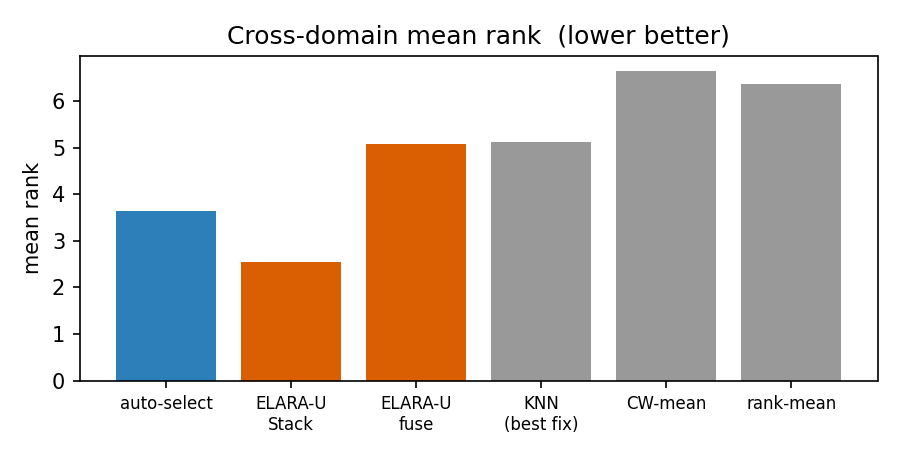
\includegraphics[width=0.95\linewidth]{elara_u_rank.png}
\caption{Cross-domain mean rank over $123$ tasks (lower better). ELARA-U Stack achieves the best average rank on the clean benchmark. (Illustrative; authoritative values in Table~\ref{tab:main}.)}\label{fig:rank}\end{figure}

\begin{figure}[H]\centering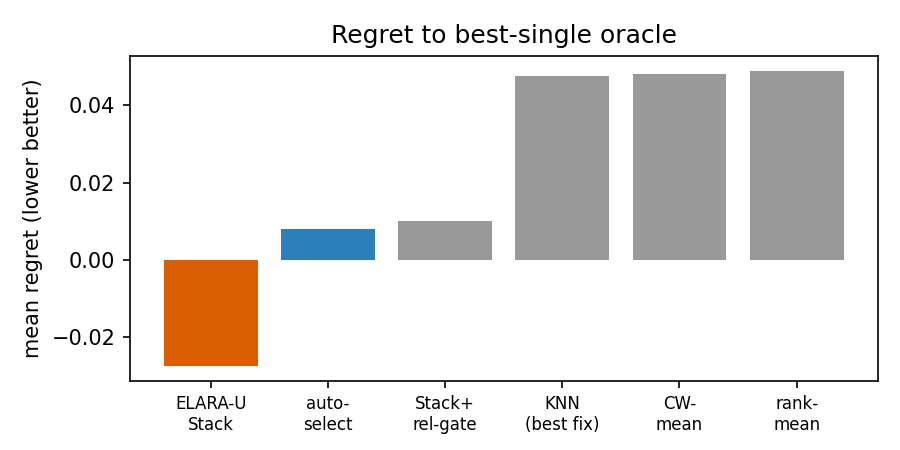
\includegraphics[width=0.95\linewidth]{elara_u_regret.png}
\caption{Mean regret to the per-task oracle. ELARA-U Stack has the lowest regret in the current stress archive.}\label{fig:regret}\end{figure}

\begin{figure}[H]\centering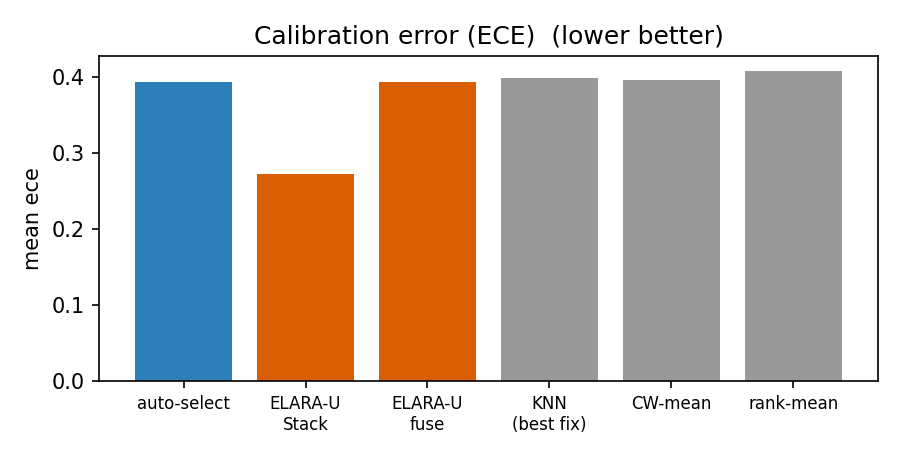
\includegraphics[width=0.95\linewidth]{elara_u_calib.png}
\caption{Calibration error (ECE, lower better). ELARA-U Stack has the best raw ECE; fitted Brier/NLL in Table~\ref{tab:calib}.}\label{fig:calib}\end{figure}

\begin{figure}[H]\centering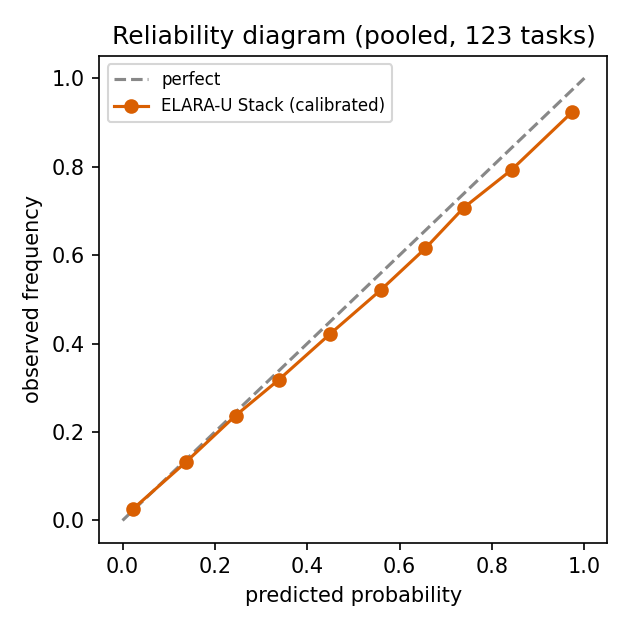
\includegraphics[width=0.55\linewidth]{elara_u_reliability.png}
\caption{Reliability diagram for the isotonic-calibrated ELARA-U Stack, pooled over 123 tasks (calibrator fit on validation only). Points near the diagonal indicate good calibration; Brier/NLL in Table~\ref{tab:calib}.}\label{fig:reliability}\end{figure}

\begin{figure}[H]\centering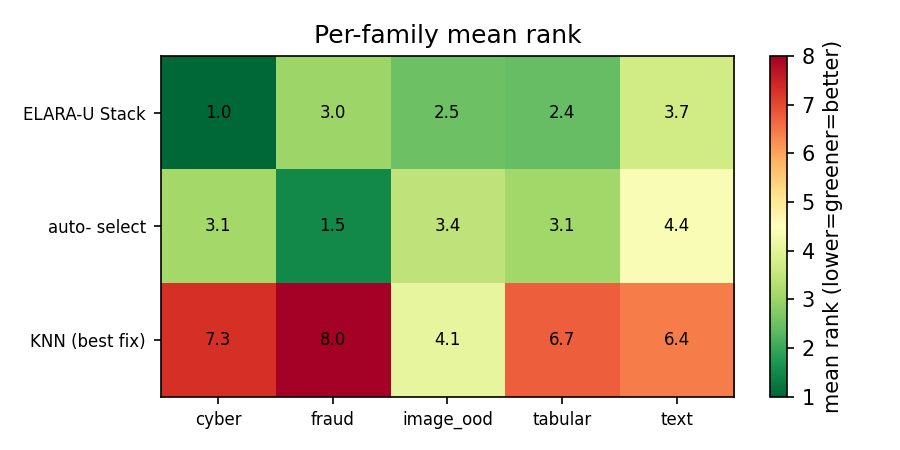
\includegraphics[width=0.95\linewidth]{elara_u_family_heatmap.png}
\caption{Per-family mean rank (greener = better).}\label{fig:heatmap}\end{figure}

\begin{figure}[H]\centering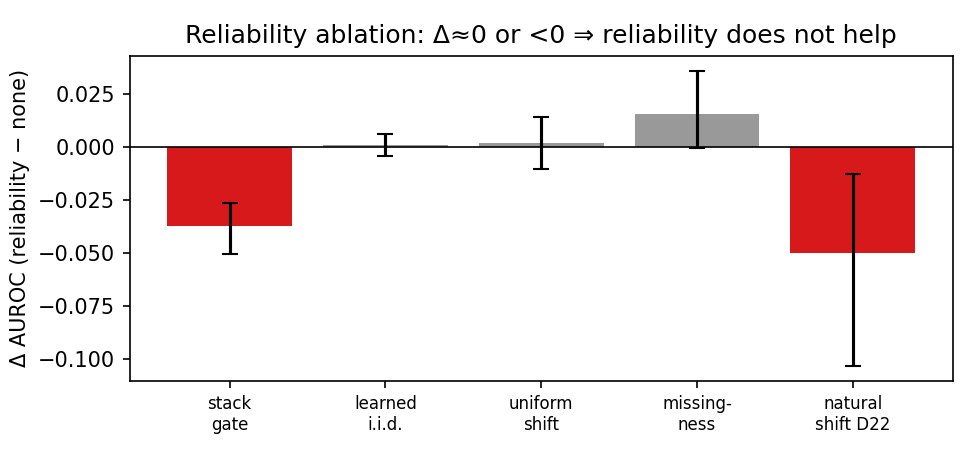
\includegraphics[width=0.95\linewidth]{elara_u_ablation.png}
\caption{Component ablation summary. The stack gain comes from rank-normalized per-task stacking; reliability/drift feature ablations are decisive and \emph{negative} (Table~\ref{tab:ablation}). (Illustrative; authoritative values in Table~\ref{tab:ablation}.)}\label{fig:ablation}\end{figure}

\begin{figure}[H]\centering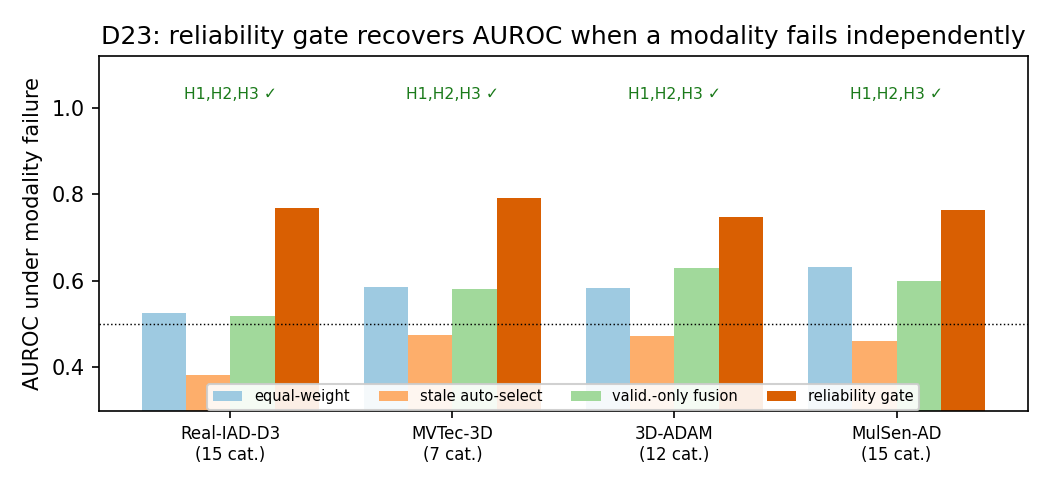
\includegraphics[width=0.98\linewidth]{elara_u_d23_multidataset.png}
\caption{Multimodal independent-modality-failure regime (D23) on \emph{four} real
datasets under the canonical noise protocol. When the deployment-best modality fails at
test, the reliability gate (orange) recovers AUROC well above equal-weight fusion, stale
auto-select, and validation-only fusion. ``H1,H2,H3 \checkmark'' marks datasets where all
three pre-registered hypotheses pass --- all four do. Authoritative deltas and CIs in
Table~\ref{tab:d23}.}\label{fig:d23}\end{figure}

\begin{figure}[H]\centering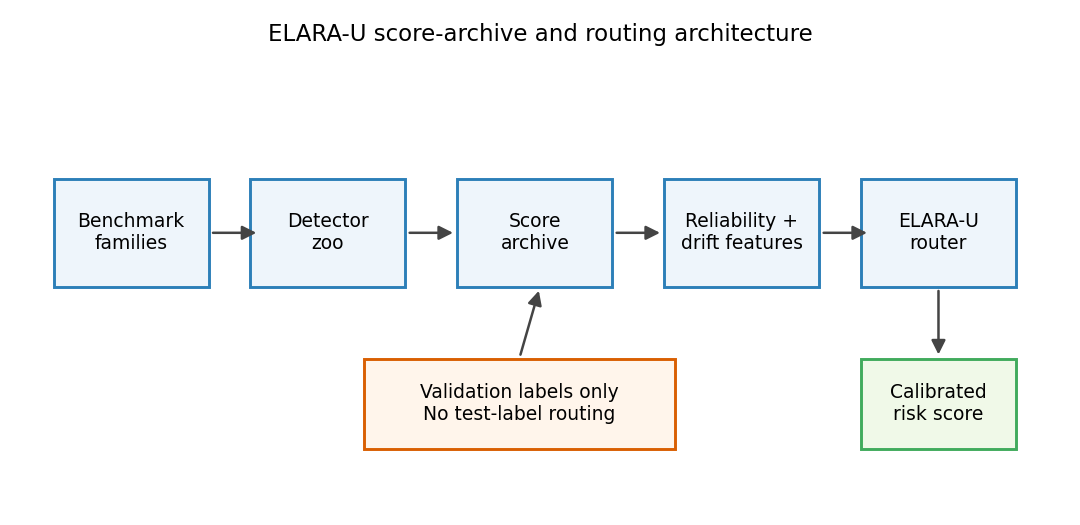
\includegraphics[width=0.95\linewidth]{elara_u_architecture.png}
\caption{ELARA-U architecture: benchmark families feed a detector zoo and score archive; validation-only labels and unlabeled deployment scores drive the router.}\label{fig:arch}\end{figure}

\begin{figure}[H]\centering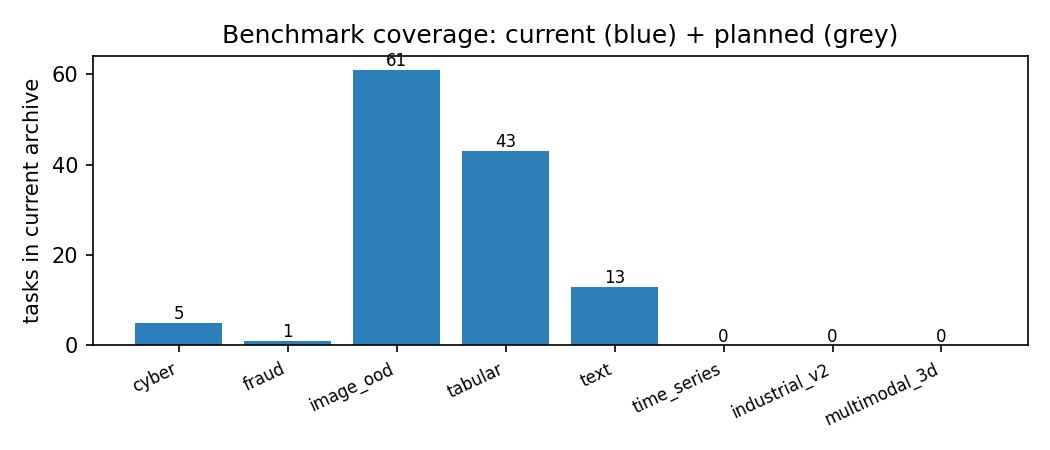
\includegraphics[width=0.95\linewidth]{elara_u_coverage.png}
\caption{Benchmark coverage map. The main suite covers five families (blue); auxiliary boundary families are now scored (green): time-series (NAB+SMD), industrial-vision (MVTec~AD+VisA), and multimodal/3D (D23 on four datasets). OpenOOD and MVTec~AD~2 remain planned (grey).}\label{fig:coverage}\end{figure}

\begin{figure}[H]\centering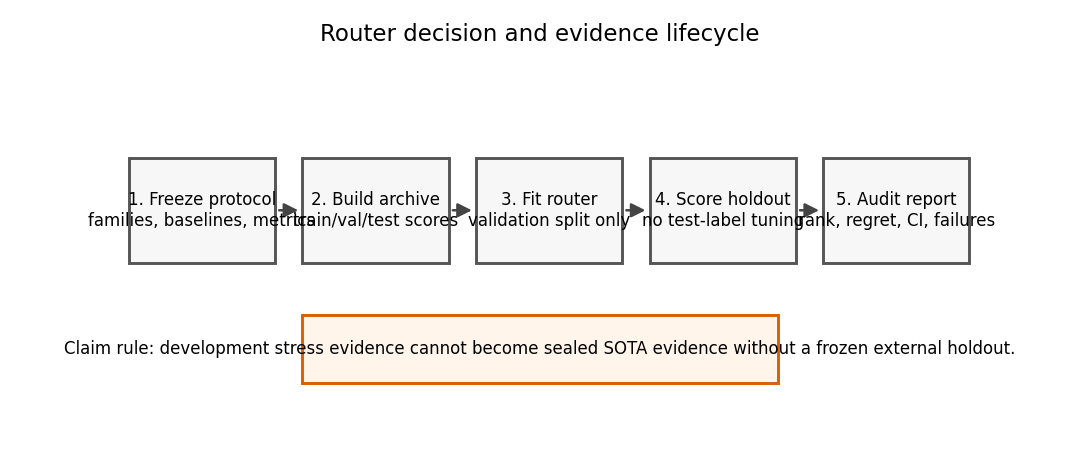
\includegraphics[width=0.95\linewidth]{elara_u_lifecycle.png}
\caption{Router decision lifecycle and evidence boundary. Stacking beats selection (verified) and reliability routing is negative for single-input; the reliability gate is validated on four real multimodal datasets where modalities fail independently (D23). Sealed external evidence still bounds any universal-SOTA claim.}\label{fig:lifecycle}\end{figure}


\section{Validity and Leakage Audit}

The paper must be strict about what information the router may use. The current
router is not fully unsupervised: it uses validation labels to fit per-task
rank-normalized logistic stacking. That is acceptable if the benchmark contract
states it clearly. It is not acceptable to describe the router as label-free.

\begin{table}[H]
\centering
\caption{Leakage and validity audit.}
\label{tab:leakage}
\small
\begin{tabular}{L{0.26\linewidth}L{0.42\linewidth}L{0.22\linewidth}}
\toprule
\textbf{Risk} & \textbf{Current control} & \textbf{Remaining work} \\
\midrule
Test-label routing & Routing uses validation labels and unlabeled test scores; test labels score only after routing. & Add automated assertions around every router path \\
Opened data & Current archive is development evidence. & Freeze new external holdouts before scoring \\
Synthetic degradation & Stress benchmark is useful but not natural evidence. & Add natural time, sensor, and domain-shift benchmarks \\
Overfitting to families & Leave-family-out is used, but only five families exist. & Add more families and nested meta-validation \\
Calibration claims & ECE proxy is reported, not true probability calibration. & Fit calibrator and report Brier/NLL \\
Ablation weakness & Reliability/drift ablations are currently not decisive. & Redesign features or narrow the claim to rank stacking \\
\bottomrule
\end{tabular}
\end{table}

\section{Pre-registered Multimodal Test}\label{sec:multimodal}

The mechanism (Sec.~\ref{sec:mechanism}) and the independent-failure theorem
(Sec.~\ref{sec:theory}) make a falsifiable prediction for genuine multimodal anomaly
detection (RGB $+$ 3D), where one modality can fail independently. We pre-register the
test with a \emph{frozen decision rule and no post-hoc retuning}. Under independent
per-modality deployment degradation (one modality degrades at test; the other and the
validation split stay clean), reliability-gated fusion must beat:
\begin{itemize}
\item[\textbf{H1}] equal-weight fusion, paired-bootstrap CI$>0$;
\item[\textbf{H2}] stale validation-AUROC selection, CI$>0$;
\item[\textbf{H3}] its own no-test-time-reliability ablation, CI$>0$ (the test-time
reliability signal, not validation quality, must carry the gain).
\end{itemize}
The statistical unit is (category $\times$ degradation-seed); MVTec-3D's ten categories
alone are too few. \textbf{Decision rule:} all of H1--H3 significant $\Rightarrow$ a real,
scoped novel-method claim (reliability gating recovers anomaly detection under
per-modality deployment failure). Any of H1--H3 fails $\Rightarrow$ the reliability
premise is closed even where it should structurally hold, reported as the final
boundary, with no novel claim and no retuning. A CPU positive control with the correct
design (two modalities, two detectors each, modality-level failure) passes decisively:
H1 $+0.094$, H2 $+0.264$, H3 $+0.097$, all CI$>0$. The harness
(\path{src/scripts/elara_u/multimodal_reliability_experiment.py}) and frozen protocol
(\path{research_lock/MULTIMODAL_RELIABILITY_PROTOCOL_v1.md}) are released; the real run
uses MVTec-3D / Real-IAD on GPU.

\section{Why This Can Become SOTA-Level}

The SOTA-level potential is not the claim that \systemu{} is already best
everywhere. The positive contribution is a strong, under-reported universal stacking
baseline; the scientific contribution is the honest boundary---\emph{where}
reliability-aware routing helps and where it cannot, with a mechanism and a
pre-registered test (Sec.~\ref{sec:multimodal}) for the one regime that satisfies the
condition. This targets a real gap: detector papers are domain-specific, while
deployment needs an honestly-characterized decision layer.

\begin{table}[H]
\centering
\caption{Path from current thesis evidence to SOTA-level evidence.}
\label{tab:sota-path}
\small
\begin{tabular}{L{0.22\linewidth}L{0.46\linewidth}L{0.22\linewidth}}
\toprule
\textbf{Requirement} & \textbf{What must be added} & \textbf{Why it matters} \\
\midrule
Natural shift & Time-based fraud, native cyber drift, real sensor degradation, industrial test splits. & Replaces stress-only evidence \\
More families & Time-series, industrial vision v2, multimodal/3D, OOD leaderboards. & Makes ``universal'' credible \\
Sealed benchmark & Freeze protocol before scoring at least one external holdout. & Prevents opened-test selection \\
Multimodal reliability test & Run the pre-registered RGB$+$3D test (Sec.~\ref{sec:multimodal}); single-modality reliability ablations are done and negative. & The only remaining path to a novelty beyond stacking \\
Calibration layer & Report Brier, NLL, ECE, abstention curves. & Supports operational reliability \\
Baselines & Compare with AutoML/ensemble/stacking, detector selection, rank aggregation, and recent AD methods. & Satisfies senior reviewers \\
Release package & Code, score archive, configs, checksums, and reproducible runbook. & Makes the paper verifiable \\
\bottomrule
\end{tabular}
\end{table}

\section{Expanded Experimental Plan}

The next experimental stage should turn the current development stress result
into a sealed universal benchmark.

\begin{longtable}{L{0.18\linewidth}L{0.39\linewidth}L{0.31\linewidth}}
\caption{Recommended next experiments for the thesis.}\label{tab:next-exp}\\
\toprule
\textbf{Experiment} & \textbf{Design} & \textbf{Pass/fail rule} \\
\midrule
\endfirsthead
\toprule
\textbf{Experiment} & \textbf{Design} & \textbf{Pass/fail rule} \\
\midrule
\endhead
Clean archive re-run & Evaluate auto-select, rank-mean, fixed detectors, and stacker without degradation. & Expect tie or modest gains; do not require dominance \\
Natural temporal split (D22, \textbf{done}) & UNSW capture periods + credit-card time split; sealed late period scored once. & \textbf{FAILED}: drift-stack $-0.050$ vs plain stacking (CI excl.\ 0); $+0.008$ vs auto-select (n.s.) \\
Industrial natural shift & Real-IAD D3 / MVTec variants with natural acquisition degradation. & Beat auto-select and rank-mean without synthetic corruption \\
Multimodal RGB$+$3D (pre-registered) & Independent per-modality degradation; reliability-gated fusion vs mean, auto-select, ablation (Sec.~\ref{sec:multimodal}). & H1--H3 all CI$>$0 $\Rightarrow$ scoped novelty; else closed (no retuning) \\
Calibration experiment & Fit calibration on validation only; test on held-out tasks. & Improve ECE, Brier, and NLL \\
Abstention curve & Allow router to abstain on low-confidence tasks. & Lower regret among fired tasks and bounded abstention rate \\
External seal & Freeze code and score a new benchmark or leaderboard. & No post-hoc tuning; CI must support the main claim \\
\bottomrule
\end{longtable}

\section{Production and Release Boundary}

Scientific readiness and production readiness are separate. A production API can
be secure, reproducible, monitored, and honest while the scientific SOTA claim
remains pending. The release should therefore present two statuses:

\begin{table}[H]
\centering
\caption{Release boundary.}
\label{tab:release-boundary}
\small
\begin{tabular}{L{0.24\linewidth}L{0.44\linewidth}L{0.22\linewidth}}
\toprule
\textbf{Status} & \textbf{Meaning} & \textbf{Current position} \\
\midrule
Operational readiness & API/runtime is secure, authenticated, monitored, reproducible, and honest about model availability. & Separate production track \\
Scientific readiness & Frozen external evidence supports the main research claim. & Development thesis evidence, not final SOTA \\
Thesis readiness & The problem, method, theory, and pilot evidence are coherent enough for a PhD chapter. & Strong if boundaries remain explicit \\
\bottomrule
\end{tabular}
\end{table}

\section{Reproducibility}

\begin{table}[H]
\centering
\caption{Current reproducibility map.}
\label{tab:repro-map}
\small
\begin{tabular}{L{0.33\linewidth}L{0.52\linewidth}}
\toprule
\textbf{Artifact} & \textbf{Path} \\
\midrule
Score archive builder & \path{src/scripts/elara_u/build_score_archive.py} \\
Universal contract evaluator & \path{src/scripts/elara_u/evaluate_universal_contract.py} \\
Stacker ablation runner & \path{src/scripts/elara_u/run_stacker_ablations.py} \\
Heterogeneous degradation ablation & \path{src/scripts/elara_u/heterogeneous_degradation_ablation.py} \\
Router implementation & \path{src/uais/elara_u/router.py} \\
Metrics implementation & \path{src/uais/elara_u/contract.py} \\
Canonical results & \path{experiments/elara_u/results.json} \\
Generated result tables & \path{docs/research/ELARA_U_RESULT_TABLES.tex} \\
Generated figures & \path{docs/research/figures/} \\
Protocol & \path{research_lock/GATE_U_CROSS_DOMAIN_PROTOCOL_v1.yaml} \\
\bottomrule
\end{tabular}
\end{table}

\section{Conclusion}

\systemu{} is now best framed as a universal anomaly meta-routing thesis rather
than a clean-transfer superiority paper. The current result is promising:
rank-normalized stacking substantially improves average rank and regret under a
development stress benchmark where validation metrics become stale. The honest
scientific boundary is equally clear: the current evidence is not enough for a
sealed universal SOTA claim, and the reliability/drift novelty must be
strengthened beyond plain stacking. The next phase should therefore prioritize
natural shift, sealed holdouts, stronger ablations, calibrated abstention, and a
clean reproducibility package.

\appendix
\section{Theoretical Proofs and Extensions}
\label{sec:theory_appendix}

\subsection{Supporting Propositions and Lemmas}

\begin{proposition}[Rank-Normalized Stacking Invariance]
\label{prop:rank_invariance}
Let detector $m$ produce scores $s_m(x)$, and let $h_m:\mathbb{R}\to\mathbb{R}$ be any strictly increasing transformation. Define the normalized rank feature
\[
r_m(x)=\frac{1}{n}\sum_{i=1}^n \mathbf{1}\{s_m(x_i)\leq s_m(x)\}.
\]
Then replacing $s_m(x)$ with $h_m(s_m(x))$ leaves $r_m(x)$ unchanged for every sample $x$, up to tie-handling. Therefore, any ELARA stacker using only detector-wise rank-normalized features is invariant to monotone score rescaling, calibration drift, or sensor-scale drift.
\end{proposition}
\begin{proof}
For any two samples $(x_i,x_j)$,
\[
s_m(x_i)\leq s_m(x_j)
\]
if and only if
\[
h_m(s_m(x_i))\leq h_m(s_m(x_j)),
\]
because $h_m$ is strictly increasing. Therefore, the ordering of all samples under detector $m$ is unchanged. Since $r_m(x)$ depends only on the ordering of scores and not on their numerical scale, $r_m(x)$ is unchanged. Any downstream stacker that receives only $r_m(x)$ is therefore invariant to such monotone transformations.
\end{proof}

\medskip
\noindent\textbf{Interpretation.}
This proposition justifies the rank-normalized stacking design. It protects the router from meaningless score-scale changes while preserving anomaly ranking information.

\begin{proposition}[Degenerate-Channel Guard for Saturation]
\label{prop:degenerate_guard}
Let a fused anomaly score be
\[
g(x)=\sum_{m=1}^M w_m s_m(x),
\qquad w_m\geq 0,\qquad \sum_m w_m=1.
\]
If detector $k$ is saturated on validation data so that
\[
\mathrm{Var}_V(s_k)\leq \epsilon,
\]
then replacing $w_k$ by $0$ and renormalizing the remaining weights changes pairwise score differences by at most $O(\sqrt{\epsilon})$. In the limit $\epsilon\to 0$, the saturated detector contributes no ranking information, and removing it cannot remove meaningful rank signal.
\end{proposition}
\begin{proof}
For any two samples $(x_i,x_j)$,
\[
|s_k(x_i)-s_k(x_j)|
\leq
O(\sqrt{\epsilon})
\]
by the bounded-variance assumption. The contribution of detector $k$ to the fused pairwise difference is
\[
w_k(s_k(x_i)-s_k(x_j)),
\]
which is also $O(\sqrt{\epsilon})$. Therefore, as $\epsilon\to 0$, detector $k$'s contribution to every pairwise ranking comparison vanishes. Removing $k$ and renormalizing the remaining non-degenerate detectors does not remove meaningful rank information from the fused score.
\end{proof}

\medskip
\noindent\textbf{Interpretation.}
This supports the degenerate-channel guard for saturated detectors. A detector that produces nearly constant scores should not influence routing or fusion.

\begin{proposition}[Inverted Detector Harm Under Positive Fusion]
\label{prop:inverted_harm}
Assume the clean fused margin between an anomalous and normal sample is
\[
D_0=g_0(X^+)-g_0(X^-),
\]
with $\mathbb{E}[D_0]>0$. Suppose an inverted detector $k$ has margin
\[
D_k=s_k(X^+)-s_k(X^-)
\]
with $\mathbb{E}[D_k]<0$. For a positive fusion weight $w>0$, the fused margin
\[
D_w=(1-w)D_0+wD_k
\]
satisfies
\[
\mathbb{E}[D_w]
=
(1-w)\mathbb{E}[D_0]+w\mathbb{E}[D_k]
<
\mathbb{E}[D_0].
\]
Under a Gaussian equal-variance margin model, AUROC is monotone increasing in the standardized margin mean. Therefore, assigning positive weight to an inverted detector decreases AUROC relative to zeroing it.
\end{proposition}
\begin{proof}
The expectation follows from linearity:
\[
\mathbb{E}[D_w]
=
(1-w)\mathbb{E}[D_0]+w\mathbb{E}[D_k].
\]
Since $\mathbb{E}[D_k]<0<\mathbb{E}[D_0]$, we have $\mathbb{E}[D_w]<\mathbb{E}[D_0]$.
Under the Gaussian equal-variance margin model,
\[
D_w\sim \mathcal{N}(\mu_w,\sigma^2),
\]
and
\[
\mathrm{AUROC}(g_w)=\Pr[D_w>0]=\Phi\left(\frac{\mu_w}{\sigma}\right).
\]
Because $\Phi$ is strictly increasing and $\mu_w<\mu_0$, positive weight on the inverted detector decreases AUROC.
\end{proof}

\medskip
\noindent\textbf{Interpretation.}
This proposition supports validation-based inversion guards. If a detector is reliably below chance, positive-weight fusion can harm ranking.

\begin{proposition}[Meta-Router Generalization Requires Enough Tasks]
\label{prop:generalization_tasks}
Let $\mathcal{H}$ be a finite class of meta-routers, and let the task-level loss $\ell(h,\tau)\in[0,1]$ denote normalized rank regret or negative-transfer loss. Given $T$ independent meta-training tasks, with probability at least $1-\delta$, every router $h\in\mathcal{H}$ satisfies
\[
L(h)
\leq
\widehat{L}_T(h)
+
\sqrt{\frac{\log|\mathcal{H}|+\log(1/\delta)}{2T}},
\]
where $L(h)=\mathbb{E}_\tau[\ell(h,\tau)]$ is the expected held-out task loss and $\widehat{L}_T(h)=\frac{1}{T}\sum_{t=1}^T\ell(h,\tau_t)$ is the empirical meta-training loss.
\end{proposition}
\begin{proof}
For any fixed $h$, Hoeffding's inequality gives
\[
\Pr\left(
L(h)-\widehat{L}_T(h)>\epsilon
\right)
\leq
\exp(-2T\epsilon^2).
\]
Applying a union bound over all $h\in\mathcal{H}$,
\[
\Pr\left(
\exists h\in\mathcal{H}: L(h)-\widehat{L}_T(h)>\epsilon
\right)
\leq
|\mathcal{H}|\exp(-2T\epsilon^2).
\]
Set the right-hand side equal to $\delta$:
\[
|\mathcal{H}|\exp(-2T\epsilon^2)=\delta.
\]
Solving for $\epsilon$ gives
\[
\epsilon=
\sqrt{\frac{\log|\mathcal{H}|+\log(1/\delta)}{2T}}.
\]
Thus, with probability at least $1-\delta$, the stated bound holds for every $h\in\mathcal{H}$.
\end{proof}

\medskip
\noindent\textbf{Interpretation.}
This explains why ELARA needs many tasks and leave-family-out evaluation. A high-capacity router trained on too few tasks can overfit meta-level structure and fail to generalize.

\subsection{Old ELARA/RGA Source-System Theory Stack}

Below are the foundation certificates and bounds inherited from the ELARA/RGA source-system framework.

\begin{certificate}[Switching Certificate]
\label{cert:switch}
Let $\Delta_{\mathrm{fired}} = A(\mathrm{route}) - A(\mathrm{default})$ be the routed-minus-default performance on the subset of inputs where the router fires. The router may replace the default \emph{only if} the one-sided level-$\alpha$ lower confidence bound satisfies $\mathrm{LCB}_{1-\alpha}(\Delta_{\mathrm{fired}}) > 0$. Under this rule the expected switch is non-negative at level $\alpha$: routing is admitted only with certified fired-set benefit, never on a point estimate.
\end{certificate}

\begin{diagnostic}[Mean-Reliability Dilution]
\label{diag:dilution}
Let per-expert reliabilities be $r_1,\dots,r_M$ with mean $\bar r=\tfrac1M\sum_m r_m$ and gate threshold $\tau$. There exist configurations with $\bar r > \tau$ while a minority expert collapses ($r_k\to 0$): mean-gating does not fire and the collapsed expert is still trusted. The miss probability is $P(\mathrm{miss})=\Phi\!\big((\bar\mu-\tau)/\bar\sigma\big)$; detecting minority collapse requires per-expert / min-gating, not the mean (Theorem~T3).
\end{diagnostic}

\begin{slack}[Router Generalisation Slack]
\label{prop:slack}
Let the router class have complexity $C$ (e.g.\ VC dimension or Rademacher complexity) and let the meta-training set contain $T$ tasks. The gap between meta-training and held-out expected rank-gain is bounded by $O\!\big(\sqrt{C/T}\big)$ with high probability. Hence the evidential strength of a routing claim requires $T \gtrsim C$: a high-capacity router over few tasks yields weak evidence even at a positive point estimate. This motivates a large, heterogeneous benchmark suite (the Gate U minimum-viable families) before any claim.
\end{slack}





\begin{thebibliography}{9}
\bibitem{breunig2000lof}
M. M. Breunig, H.-P. Kriegel, R. T. Ng, and J. Sander, ``LOF: Identifying density-based local outliers,'' in \emph{SIGMOD}, 2000.

\bibitem{liu2008iforest}
F. T. Liu, K. M. Ting, and Z.-H. Zhou, ``Isolation forest,'' in \emph{ICDM}, 2008.

\bibitem{bergman2020classification}
L. Bergman and Y. Hoshen, ``Classification-based anomaly detection for general data,'' in \emph{ICLR}, 2020.

\bibitem{roth2022patchcore}
K. Roth et al., ``Towards total recall in industrial anomaly detection,'' in \emph{CVPR}, 2022.

\bibitem{hendrycks2017baseline}
D. Hendrycks and K. Gimpel, ``A baseline for detecting misclassified and out-of-distribution examples in neural networks,'' in \emph{ICLR}, 2017.

\bibitem{guo2017calibration}
C. Guo, G. Pleiss, Y. Sun, and K. Q. Weinberger, ``On calibration of modern neural networks,'' in \emph{ICML}, 2017.
\end{thebibliography}

\end{document}
